% ============================================================
%  Chapter 1 — The Travelling Salesperson Problem
%  Nature Inspired Optimisation for Delivery Problems (2022)
%  Self-contained Beamer slides (reader-friendly, prose style)
% ============================================================
\documentclass[aspectratio=169,10pt]{beamer}

\usetheme{Madrid}
\usecolortheme{seahorse}

% ── Packages ────────────────────────────────────────────────
\usepackage{graphicx}
\usepackage{amsmath,amssymb}
\usepackage{booktabs}
\usepackage{array}
\usepackage{listings}
\usepackage{xcolor}
\usepackage{tikz}
\usepackage{microtype}
\usepackage{lmodern}

\graphicspath{{figures/}}

% ── Listings style ──────────────────────────────────────────
\lstset{
  language=Python,
  basicstyle=\ttfamily\scriptsize,
  numbers=left,
  numberstyle=\tiny\color{gray},
  frame=single,
  backgroundcolor=\color{gray!7},
  commentstyle=\color{green!50!black}\itshape,
  keywordstyle=\color{blue!70!black}\bfseries,
  stringstyle=\color{orange!80!black},
  breaklines=true,
  tabsize=4,
  showstringspaces=false,
  xleftmargin=1.5em,
  framexleftmargin=1.5em,
}

% ── Footline ────────────────────────────────────────────────
\setbeamertemplate{footline}[frame number]

% ── Title info ──────────────────────────────────────────────
\title[Chapter 1: TSP]{Chapter 1\\The Travelling Salesperson Problem}
\subtitle{Nature Inspired Optimisation for Delivery Problems (2022)}
\author{Slides based on the textbook}
\date{2022}

% ============================================================
\begin{document}
% ============================================================

% ── Title slide ─────────────────────────────────────────────
\begin{frame}
  \titlepage
\end{frame}

% ── Contents ────────────────────────────────────────────────
\begin{frame}{Chapter Overview}
  \tableofcontents
\end{frame}

% ============================================================
\section{1.1~~A Brief History of the TSP}
% ============================================================

\begin{frame}[allowframebreaks]{1.1~~A Brief History of the TSP}

  The \textbf{Travelling Salesperson Problem} (TSP) is one of the most
  famous and extensively studied combinatorial optimisation problems in
  mathematics and computer science.  Although it sounds simple --- visit a
  set of cities, return home, minimise the total distance travelled --- it
  has proved extraordinarily difficult to solve in general, and that
  difficulty has motivated decades of algorithmic research.

  \medskip
  \textbf{Origins.}
  The problem was first described in mathematical terms by the Irish
  mathematician \textbf{W.~R.~Hamilton} and the British mathematician
  \textbf{Thomas Kirkman} in the 1800s.  Hamilton posed the ``Icosian Game''
  (1857), which asked for a Hamiltonian circuit --- a closed path that
  visits every vertex of a graph exactly once --- on the edges of an
  icosahedron.

  \medskip
  \textbf{The name and modern formulation.}
  The term ``Travelling Salesman Problem'' was introduced by
  \textbf{Merrill Flood} and \textbf{Melvin Dresher} at the RAND
  Corporation in the 1940s.  \textbf{Karl Menger} had already noted in
  Vienna in the 1930s that na\"{\i}ve exhaustive search would be
  computationally infeasible even for moderate-sized instances.

  \medskip
  \textbf{Key milestone.}
  The first computerised solution appeared in 1958: \textbf{Bocks (1958)}
  described solving the TSP using an algorithm implemented on an
  \textbf{IBM~650} computer, marking the beginning of the computational
  era for combinatorial optimisation.

  \medskip
  \textbf{Why the TSP remains important.}
  The TSP is important not merely for routing salespeople.  Because it
  captures the essence of NP-hard combinatorial search, virtually every
  delivery, logistics, or routing problem in the modern world inherits
  the TSP's difficulty.  Progress on the TSP --- exact methods,
  heuristics, metaheuristics --- directly translates into better
  algorithms for vehicle routing, circuit board drilling, genome
  sequencing, and telescope scheduling.

\end{frame}

% ============================================================
\section{1.2~~Problem Description}
% ============================================================

\begin{frame}[allowframebreaks]{1.2~~Problem Description}

  \begin{block}{Informal problem statement}
    A salesperson must visit a number of cities, each city visited
    \emph{exactly once}, with the salesperson ending back at the starting
    city.  The aim is to find the \emph{shortest route} that permits all
    visits.
  \end{block}

  \medskip
  The core challenge is that we must search over all possible orderings
  (permutations) of the cities in order to find the best one.  Such
  orderings are also called \textbf{Hamiltonian circuits}, named after
  the mathematician W.~R.\ Hamilton mentioned in the previous section.

\framebreak

  \textbf{Formal elements of the TSP.}

  \begin{itemize}
    \item \textbf{Nodes (cities):} A set $V = \{v_1, v_2, \ldots, v_n\}$
      of $n$ locations that must all be visited.  Here $n$ (Roman letter
      ``n'') denotes the total number of cities.
    \item \textbf{Edges:} A set $E$ of connections between pairs of
      cities.  In the \emph{complete} TSP every city is directly
      reachable from every other city, so $E$ contains all $n(n-1)/2$
      possible pairs.
    \item \textbf{Distance matrix:} A two-dimensional table $D$ where the
      entry $d(i,j)$ gives the distance (or cost) of travelling directly
      from city~$i$ to city~$j$.  When distances are symmetric ---
      $d(i,j) = d(j,i)$ for all pairs --- the problem is called a
      \emph{symmetric} TSP.
  \end{itemize}

\framebreak

  \begin{block}{Objective function}
    Given a tour $\pi = (\pi_1, \pi_2, \ldots, \pi_n)$ --- a permutation
    ($\pi$, pronounced ``pi'') of the $n$ cities --- the total tour
    length is:
    \[
      L(\pi) \;=\;
        \sum_{i=1}^{n-1} d(\pi_i,\, \pi_{i+1})
        \;+\; d(\pi_n,\, \pi_1)
    \]
  \end{block}

  \begin{block}{Notation explained}
    \begin{itemize}
      \item $\pi$ (pi): a particular ordering of all cities, e.g.\
        $\pi = (A, C, B, D, E)$ means ``visit A first, then C, then B,
        \ldots''.
      \item $\pi_i$: the city at position $i$ in the tour.
        $\pi_1$ is the first city, $\pi_n$ is the last city before
        returning home.
      \item $d(\pi_i, \pi_{i+1})$: the distance between the $i$-th and
        $(i+1)$-th city in the tour.
      \item $\sum_{i=1}^{n-1}$ (Sigma, meaning ``sum over $i$ from 1 to
        $n-1$''): we add up all the leg distances as we traverse the
        tour, then add the final return leg $d(\pi_n, \pi_1)$.
    \end{itemize}
  \end{block}

  \begin{alertblock}{How to read this formula}
    The formula simply says: add up the distances of all the segments of
    the journey.  If you double the number of stops (roughly) and each
    leg has a similar length, the total distance roughly doubles.  The
    goal is to find the ordering~$\pi$ that makes $L(\pi)$ as small as
    possible.
  \end{alertblock}

\framebreak

  \begin{figure}
    \centering
    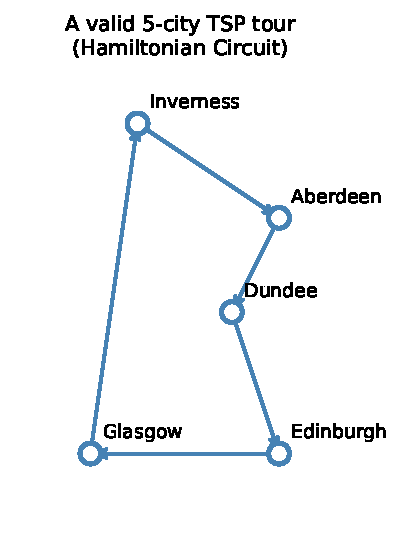
\includegraphics[width=0.45\textwidth]{fig_5city_tour.pdf}
    \caption{A valid 5-city TSP tour visiting Inverness, Aberdeen,
    Dundee, Edinburgh, and Glasgow before returning to the start.
    The arrows show the direction of travel.  There are $5! / 2 = 60$
    distinct tours on 5~cities; this is just one of them.}
  \end{figure}

\framebreak

  \begin{figure}
    \centering
    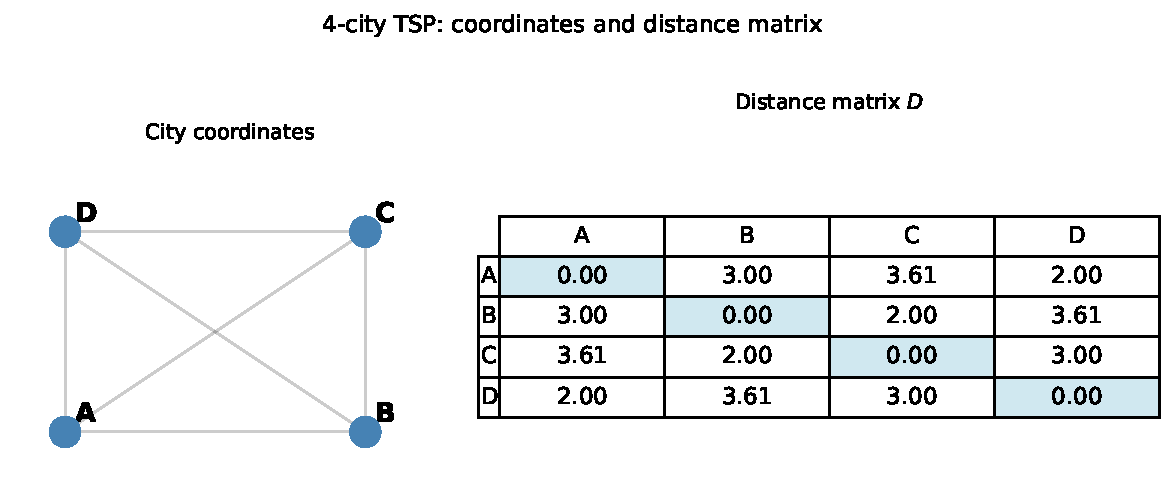
\includegraphics[width=0.70\textwidth]{fig_distance_matrix.pdf}
    \caption{A 4-city TSP example.  \emph{Left:} the cities placed on a
    grid with coordinates.  \emph{Right:} the symmetric distance matrix
    $D$ computed as Euclidean distances.  For example, the distance from
    city~A at $(0,0)$ to city~C at $(3,2)$ is
    $\sqrt{3^2 + 2^2} = \sqrt{13} \approx 3.61$.}
  \end{figure}

\framebreak

  \textbf{How many tours are there?}

  Because the tour is a \emph{permutation} of all cities and the
  starting point does not matter (the tour is circular), the number of
  distinct tours on $n$ cities is:
  \[
    \text{Number of distinct tours} \;=\; \frac{(n-1)!}{2}
  \]
  The factor $(n-1)!$ (``$(n-1)$ factorial'', the product of all
  integers from 1 up to $n-1$) accounts for fixing one city as the
  start.  The division by 2 accounts for the fact that a tour and its
  reverse are the same route.

  \medskip
  \begin{exampleblock}{Worked example: how the numbers grow}
    \begin{tabular}{rll}
      \toprule
      Cities $n$ & $(n-1)!/2$ & Comment \\
      \midrule
      5  & 12 & Trivially enumerable \\
      10 & 181\,440 & Still feasible with exhaustive search \\
      15 & $\approx 4.36 \times 10^{10}$ & About 43 billion tours --- impractical \\
      20 & $\approx 6.08 \times 10^{16}$ & More tours than grains of sand on Earth \\
      \bottomrule
    \end{tabular}
  \end{exampleblock}

  Notice that adding just a few extra cities causes the number of tours
  to increase astronomically.  This \textbf{combinatorial explosion}
  is the central challenge of the TSP.

\framebreak

  \begin{figure}
    \centering
    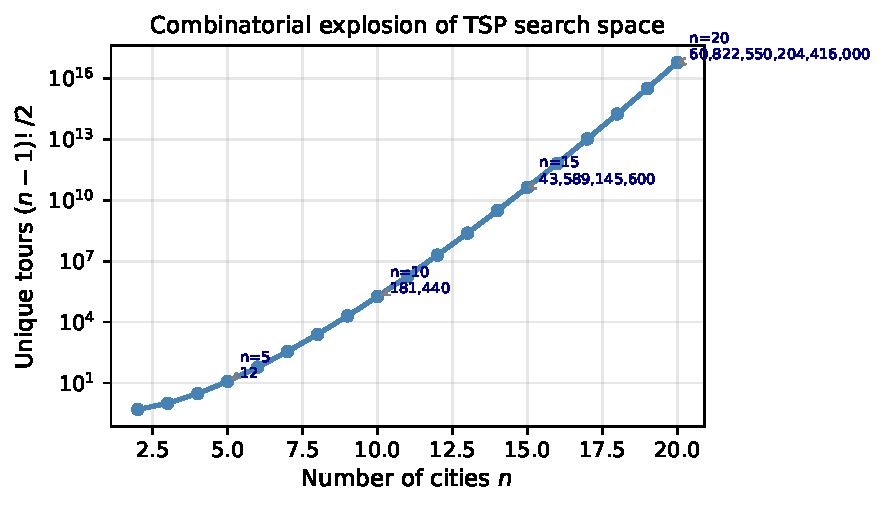
\includegraphics[width=0.72\textwidth]{fig_factorial_growth.pdf}
    \caption{The number of distinct tours grows as $(n-1)!/2$, plotted
    on a log scale.  For $n = 20$ cities the number already exceeds
    $6 \times 10^{16}$, illustrating why exhaustive search quickly
    becomes infeasible and why heuristic methods are essential.}
  \end{figure}

\framebreak

  \textbf{NP-hardness of the TSP.}

  Computer scientists classify problems by how their difficulty scales
  with input size.  The most relevant classes here are:

  \begin{itemize}
    \item \textbf{P} (Polynomial time): Problems solvable by an
      algorithm whose running time grows as a polynomial in the input
      size.  Sorting a list is in P.
    \item \textbf{NP} (Non-deterministic Polynomial time): Problems
      whose \emph{solutions} can be \emph{verified} in polynomial time,
      even if finding the solution may be hard.
    \item \textbf{NP-hard}: Problems at least as hard as any problem in
      NP.  The TSP (decision version) is NP-complete, meaning it is both
      in NP and NP-hard.
  \end{itemize}

  \begin{alertblock}{Key insight: what NP-hardness means in practice}
    No algorithm is known that solves every TSP instance in polynomial
    time.  The best exact algorithms (such as Branch and Bound and
    Concorde) use exponential time in the worst case.  For large $n$,
    we therefore rely on \emph{heuristics} --- algorithms that find good
    (but not necessarily optimal) solutions in reasonable time.
  \end{alertblock}

\framebreak

  \begin{figure}
    \centering
    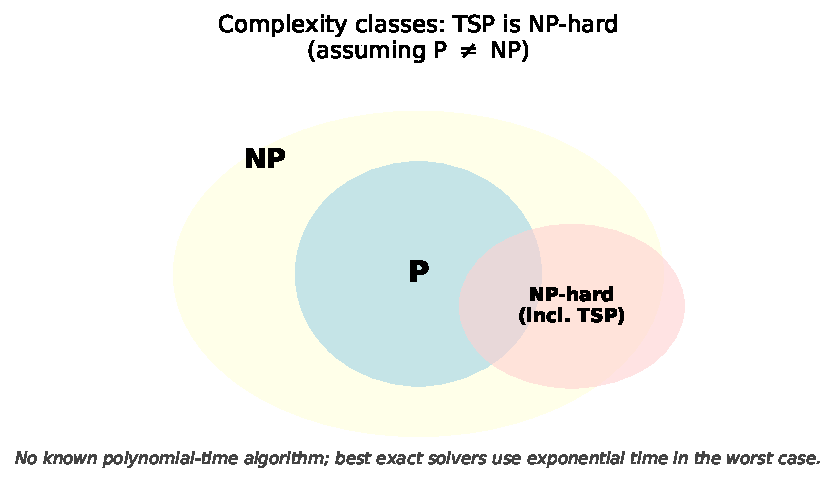
\includegraphics[width=0.55\textwidth]{fig_np_hardness.pdf}
    \caption{The complexity landscape (assuming P $\neq$ NP).  The TSP
    sits in NP-hard: solutions can be verified quickly, but finding the
    optimum requires, in the worst case, examining an exponential number
    of candidates.}
  \end{figure}

\end{frame}

% ============================================================
\section{1.3~~Techniques for Solving the TSP}
% ============================================================

\begin{frame}[allowframebreaks]{1.3~~Techniques for Solving the TSP — Overview}

  Because the TSP is NP-hard, practitioners use a spectrum of methods
  that trade \emph{solution quality} for \emph{computation time}:

  \begin{block}{Taxonomy of TSP solvers}
    \begin{description}
      \item[Exact methods] Guarantee the optimal solution but may require
        exponential time.  Practical only for small instances or with
        very sophisticated bounding.  Examples: \textbf{exhaustive
        search}, \textbf{Branch and Bound}, \textbf{Concorde} (LP + cutting
        planes).
      \item[Construction heuristics] Build a tour from scratch using a
        greedy rule.  Fast, but the result may be far from optimal.
        Example: \textbf{Nearest Neighbour}.
      \item[Improvement heuristics] Start with any tour and repeatedly
        modify it to get a shorter one.  Examples: \textbf{2-opt},
        \textbf{3-opt}, \textbf{Lin-Kernighan}.
      \item[Metaheuristics] Higher-level strategies that guide local
        search to escape local optima.  Examples: \textbf{Evolutionary
        Algorithms}, \textbf{Simulated Annealing}, \textbf{Ant Colony
        Optimisation}.
    \end{description}
  \end{block}

  The remainder of Section~1.3 focuses on methods implemented in this
  chapter's case study: Exhaustive Search, Nearest Neighbour, and 2-opt.

\end{frame}

% ────────────────────────────────────────────────────────────
\begin{frame}[allowframebreaks]{Exhaustive Search}

  \textbf{What problem it solves.}
  Exhaustive search (also called \emph{brute-force search}) enumerates
  every possible tour, measures its length, and keeps track of the
  shortest one found.  It is the only method that \emph{guarantees} the
  globally optimal solution --- because it checks all possibilities.

  \medskip
  \textbf{Why it eventually fails.}
  As we saw, the number of distinct tours is $(n-1)!/2$.  For 13~cities
  this is about 3~billion, and for 20~cities it is about $6 \times
  10^{16}$.  Even at a billion tours per second, 20~cities would take
  more than 60 million years.  Therefore exhaustive search is only
  practical for very small instances (roughly $n \leq 12$).

  \begin{block}{Algorithm 1: Exhaustive Search (pseudocode)}
    \begin{tabbing}
      \hspace{2em}\=\hspace{2em}\=\hspace{2em}\= \\
      1: \> $\mathit{notVisited} \leftarrow \{1, \ldots, n\}$ \\
      2: \> $\mathit{solution} \leftarrow \emptyset$ \\
      3: \> \textbf{for each} permutation $\pi$ of $\mathit{notVisited}$ \textbf{do} \\
      4: \>\> \textbf{if} $\mathrm{dist}(\pi) < \mathrm{dist}(\mathit{solution})$ \textbf{then} \\
      5: \>\>\> $\mathit{solution} \leftarrow \pi$ \\
      6: \> \textbf{return} $\mathit{solution}$
    \end{tabbing}
  \end{block}

  In practice, the permutations are generated \emph{recursively} (see
  the Java listing in the case study): the \texttt{search(visits, l, r)}
  function swaps elements at positions \texttt{l} through \texttt{r} to
  enumerate all orderings without storing them all in memory at once.

\framebreak

  \begin{figure}
    \centering
    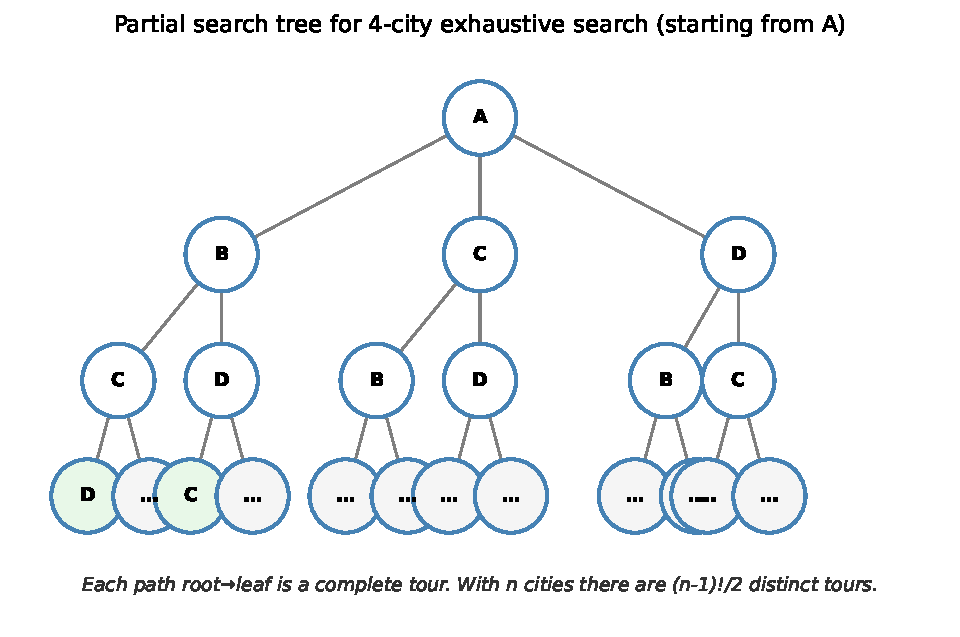
\includegraphics[width=0.65\textwidth]{fig_exhaustive_tree.pdf}
    \caption{A partial search tree for exhaustive TSP search on 4~cities
    starting from city~A.  Each path from the root to a leaf represents
    one complete tour.  With 4~cities there are $(4-1)!/2 = 3$ distinct
    tours; with $n = 15$ there are already $\approx 43$ billion.}
  \end{figure}

\end{frame}

% ────────────────────────────────────────────────────────────
\begin{frame}[allowframebreaks]{The Nearest Neighbour Heuristic}

  \textbf{What problem it solves.}
  The Nearest Neighbour (NN) heuristic is a \emph{construction heuristic}
  --- it builds a complete tour from scratch, one city at a time.  At
  each step it simply visits the \emph{closest unvisited city}.  This
  greedy strategy is intuitive and very fast, running in $O(n^2)$ time
  (quadratic in the number of cities).

  \medskip
  \textbf{Intuition: why it works reasonably well.}
  By always going to the nearest unvisited city, the salesperson avoids
  very long ``wasted'' legs.  However, because no look-ahead is
  performed, the algorithm can paint itself into a corner at the end ---
  the last few cities added to the tour may require long detours,
  making the final tour sub-optimal.  Figure~1.2 of the book illustrates
  exactly this phenomenon on a 7-city example.

  \begin{block}{Algorithm 2: TSP --- Nearest Neighbour}
    \begin{tabbing}
      \hspace{2em}\=\hspace{2em}\=\hspace{2em}\= \\
      1: \> $\mathit{notVisited} \leftarrow \{1, \ldots, n\}$ \\
      2: \> $\mathit{solution} \leftarrow \emptyset$ \\
      3: \> $\mathit{current} \leftarrow \mathrm{removeRand}(\mathit{notVisited})$
                \quad \textit{// pick a random starting city} \\
      4: \> $\mathit{solution} \leftarrow \mathit{solution} \cup \{\mathit{current}\}$ \\
      5: \> \textbf{while} $\mathit{notVisited} \neq \emptyset$ \textbf{do} \\
      6: \>\> $\mathit{best} \leftarrow \infty$ \\
      7: \>\> \textbf{for} $\mathit{possible}$ in $\mathit{notVisited}$ \textbf{do} \\
      8: \>\>\> \textbf{if} $\mathrm{dist}(\mathit{current}, \mathit{possible}) < \mathit{best}$ \textbf{then} \\
      9: \>\>\>\> $\mathit{next} \leftarrow \mathit{possible}$ \\
      10:\>\> $\mathit{notVisited} \leftarrow \mathit{notVisited} - \{\mathit{next}\}$ \\
      11:\>\> $\mathit{solution} \leftarrow \mathit{solution} \cup \{\mathit{next}\}$ \\
      12:\>\> $\mathit{current} \leftarrow \mathit{next}$ \\
      13:\> \textbf{return} $\mathit{solution}$
    \end{tabbing}
  \end{block}

  \textbf{Line-by-line explanation.}
  Line~3 picks a random starting city (making the algorithm
  \emph{stochastic}).  The main loop (lines~5--12) runs until all cities
  have been added.  Lines~7--9 scan every unvisited city to find the
  one closest to the current position.  Lines~10--12 mark it as visited,
  add it to the tour, and move there.

\framebreak

  \begin{figure}
    \centering
    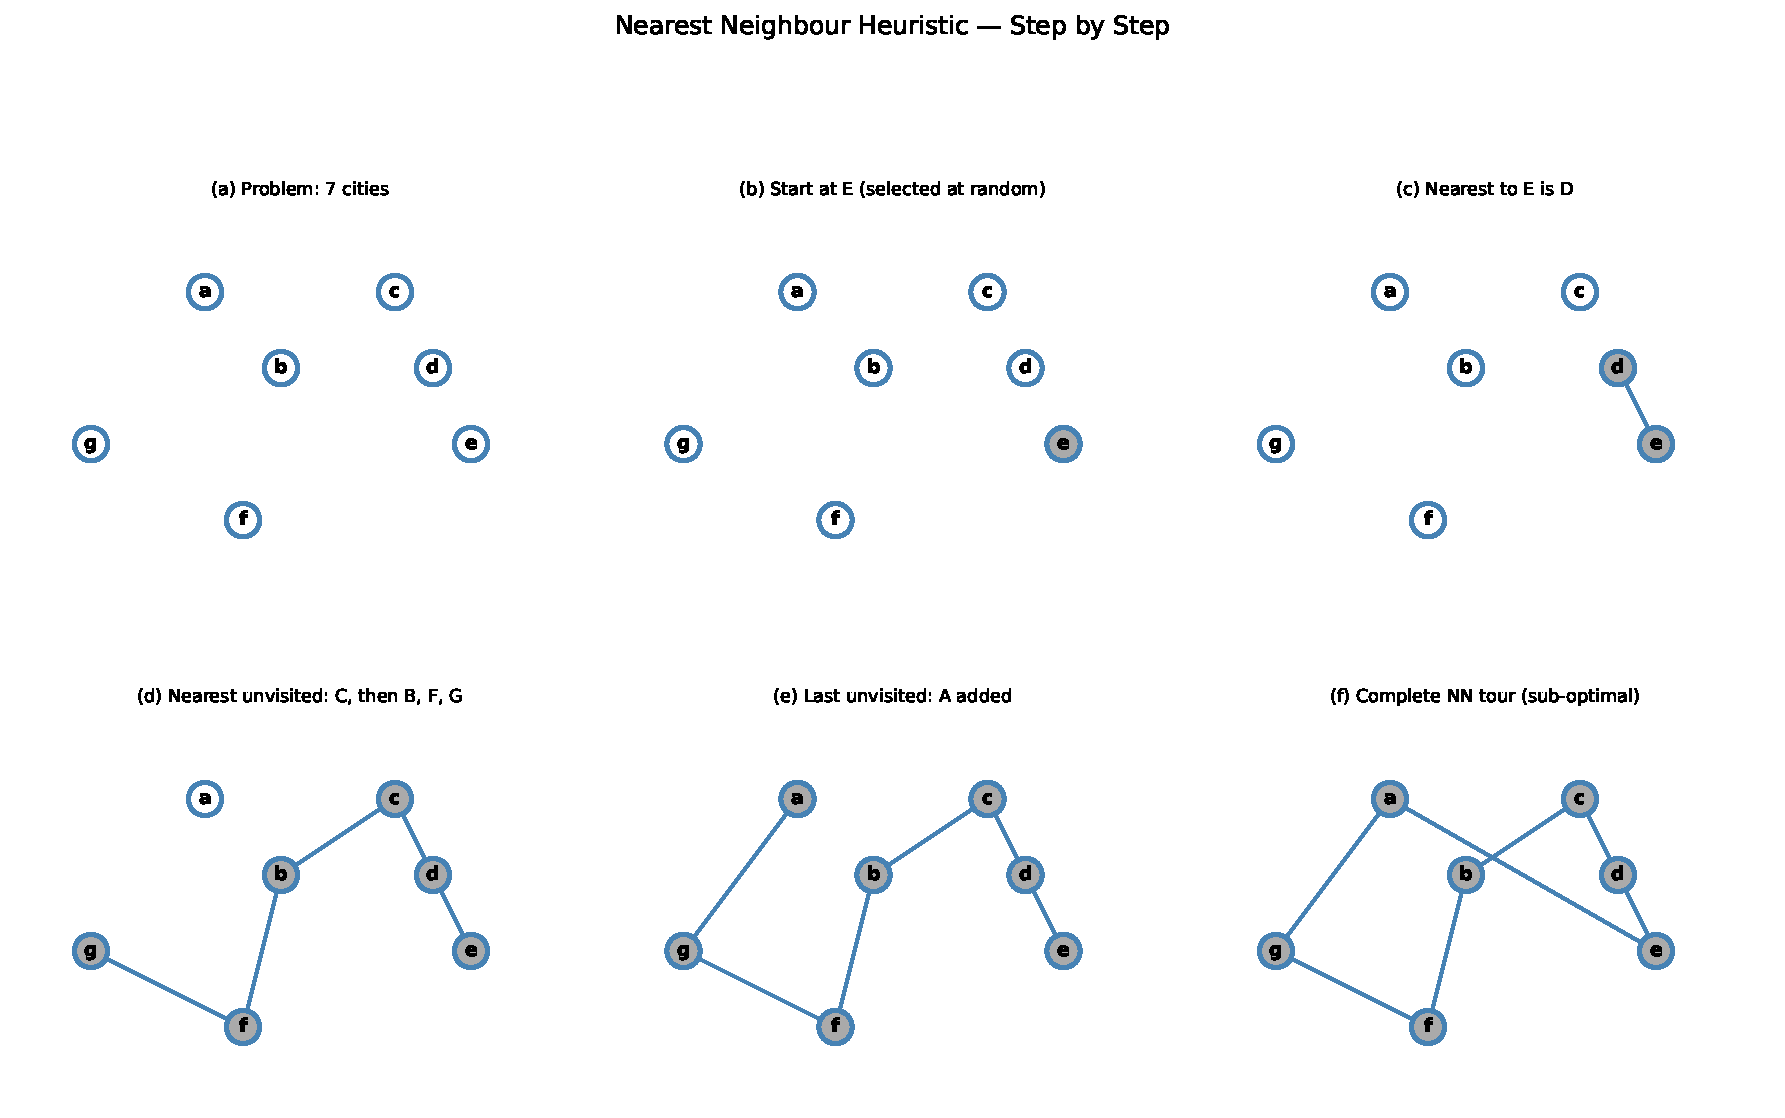
\includegraphics[width=0.80\textwidth]{fig_nn_steps.pdf}
    \caption{The Nearest Neighbour heuristic applied step by step to
    7~cities (a--g).  Starting from~e, the algorithm greedily visits d,
    then c, b, f, g, and finally the remaining city~a.  The resulting
    tour is visibly sub-optimal: the last segment (g$\to$a$\to$e)
    crosses earlier edges.  Running NN multiple times from different
    random starting cities and keeping the best result partially
    mitigates this problem.}
  \end{figure}

\framebreak

  \textbf{Stochastic vs.\ deterministic behaviour.}
  When a starting city is chosen \emph{at random}, two runs of NN on the
  same problem can produce different tours.  This is called
  \textbf{stochastic} behaviour.  Some variants of the TSP fix the
  starting city, making the algorithm \textbf{deterministic} --- the
  same input always produces the same output.  In the case study of
  Section~1.5, NN is run from the depot (fixed start), so it is
  deterministic and only needs to run once.

  \begin{alertblock}{Key takeaway: Nearest Neighbour}
    NN is fast ($O(n^2)$) and easy to implement, and its solutions are
    typically 20--25\% longer than the true optimum.  It is most useful
    as an \emph{initialisation step} for more sophisticated improvement
    heuristics such as 2-opt.
  \end{alertblock}

\end{frame}

% ────────────────────────────────────────────────────────────
\begin{frame}[allowframebreaks]{The 2-opt Heuristic}

  \textbf{What problem it solves.}
  The 2-opt heuristic (Croes 1958) is a \emph{local search} improvement
  algorithm.  It starts from an existing tour (e.g., one produced by NN)
  and repeatedly \emph{improves} it.  At each step it tries removing two
  edges from the tour and reconnecting the two resulting segments in the
  only other possible way.  If the reconnection produces a shorter tour,
  it is accepted.  The process repeats until no 2-edge swap can improve
  the tour further.

  \medskip
  \textbf{Intuition: why it works.}
  An inefficient tour often contains \emph{crossing edges} --- two edges
  that intersect in the plane.  Whenever two edges cross, swapping them
  (reversing the segment between the two crossing points) always yields a
  shorter tour.  The 2-opt algorithm systematically finds and fixes these
  crossings.

\framebreak

  \begin{figure}
    \centering
    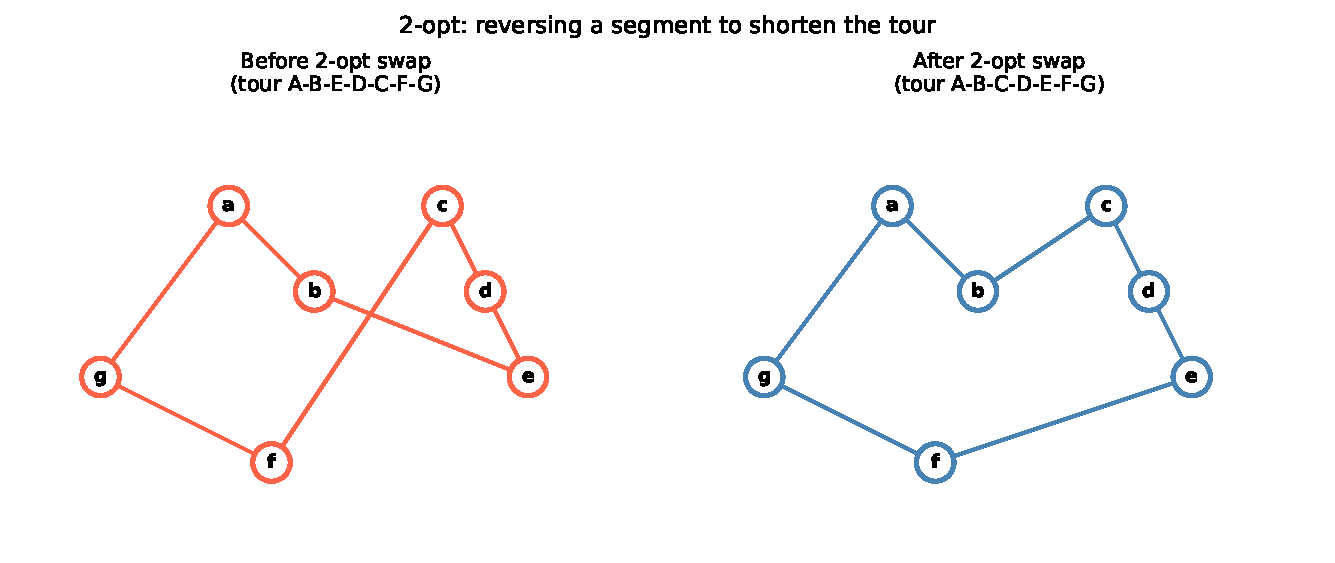
\includegraphics[width=0.72\textwidth]{fig_2opt_swap.pdf}
    \caption{A 7-city example of the 2-opt swap.
    \emph{Left:} the tour A-B-E-D-C-F-G contains two crossing edges.
    \emph{Right:} after reversing the sub-segment between the crossing
    points (reversing E-D-C to C-D-E), the edges no longer cross and
    the total tour length decreases.}
  \end{figure}

\framebreak

  \textbf{The 2-opt swap operation.}
  Given positions $i$ and $j$ in the tour (with $i < j$), the
  \emph{2-opt swap} reverses the sub-sequence between positions $i$ and
  $j$.

  \begin{exampleblock}{Worked example: 2-opt swap on a 10-city tour}
    Original tour:\quad \texttt{A B C D E F G H I J}

    We select positions $i=4$ and $j=8$ (0-indexed), highlighted:
    \quad \texttt{A B C \textbf{D E F G H} I J}

    Applying the swap reverses the bold segment:
    \quad \texttt{A B C \textbf{H G F E D} I J}

    The new tour is \texttt{A B C H G F E D I J}.
    If the total distance of this new tour is less than the original, we
    accept it; otherwise we discard it and try the next pair $(i,j)$.
  \end{exampleblock}

  The complete 2-opt algorithm (Algorithm~5 in the book) tries every
  pair of positions $(i, j)$ with $0 \leq i < j < n$, which gives
  $\binom{n}{2}$ possible swaps.  If any swap improves the tour, it is
  adopted and the scan restarts.  The algorithm terminates when a full
  scan produces no improvement.

\framebreak

  \begin{block}{Algorithm 4: 2-opt swap procedure}
    \begin{tabbing}
      \hspace{2em}\=\hspace{2em}\=\hspace{2em}\= \\
      \textbf{Procedure} $\mathrm{swap}(\mathit{tour}, i, j)$: \\
      1: \> \textbf{for} $x = 0;\; x < i;\; x{+}{+}$ \textbf{do} \\
      2: \>\> $\mathit{result}[x] \leftarrow \mathit{tour}[x]$
                \quad // copy first segment unchanged \\
      3: \> \textbf{for} $x = j;\; x \geq i;\; x{-}{-}$ \textbf{do} \\
      4: \>\> $\mathit{result}[x] \leftarrow \mathit{tour}[x]$
                \quad // copy middle segment in reverse \\
      5: \> \textbf{for} $x = j{+}1;\; x < \mathit{tour.length};\; x{+}{+}$ \textbf{do} \\
      6: \>\> $\mathit{result}[x] \leftarrow \mathit{tour}[x]$
                \quad // copy trailing segment unchanged \\
      7: \> \textbf{return} $\mathit{result}$
    \end{tabbing}
  \end{block}

  \begin{block}{Algorithm 5: Full 2-opt}
    \begin{tabbing}
      \hspace{2em}\=\hspace{2em}\=\hspace{2em}\= \\
      1: \> $\mathit{solution} \leftarrow \mathrm{randomSolution}()$ \\
      2: \> $\mathit{finished} \leftarrow \mathrm{false}$ \\
      3: \> \textbf{do} \\
      4: \>\> $\mathit{improved} \leftarrow \mathrm{false}$ \\
      5: \>\> \textbf{for} $x = 0;\; x < n;\; x{+}{+}$ \textbf{do} \\
      6: \>\>\> \textbf{for} $y = x{+}1;\; y < n;\; y{+}{+}$ \textbf{do} \\
      7: \>\>\>\> $\mathit{solution'} \leftarrow \mathrm{swap}(\mathit{solution}, x, y)$ \\
      8: \>\>\>\> \textbf{if} $\mathrm{dist}(\mathit{solution'}) < \mathrm{dist}(\mathit{solution})$ \textbf{then} \\
      9: \>\>\>\>\> $\mathit{solution} \leftarrow \mathit{solution'}$;
                    $\mathit{improved} \leftarrow \mathrm{true}$; \textbf{break} \\
      10:\> \textbf{while} $\mathit{improved}$ \\
      11:\> \textbf{return} $\mathit{solution}$
    \end{tabbing}
  \end{block}

  \textbf{Line-by-line explanation of Algorithm~5.}
  Line~1 starts from a random (or NN-generated) tour.
  The outer \textbf{do-while} loop (lines~3--10) keeps running as long
  as at least one improvement was found in the previous scan.
  Lines~5--6 iterate over all pairs $(x,y)$ of positions.
  Line~7 creates the swapped tour.
  Line~8 checks whether the swap reduces the total distance; if so,
  line~9 adopts the new tour, sets the \texttt{improved} flag, and
  breaks out of the inner loops to restart the scan from the beginning.
  When a complete scan (all $\binom{n}{2}$ pairs) finds no improvement,
  the algorithm has reached a \emph{local optimum} and terminates.

\framebreak

  \begin{block}{The iterative improvement pattern (Algorithm 3)}
    \begin{tabbing}
      \hspace{2em}\=\hspace{2em}\=\hspace{2em}\= \\
      1: \> $\mathit{solution} \leftarrow \mathrm{randomSolution}()$ \\
      2: \> \textbf{while} $\neg \mathit{done}$ \textbf{do} \\
      3: \>\> $\mathit{solution'} \leftarrow \mathrm{randomChange}(\mathit{solution})$ \\
      4: \>\> \textbf{if} $\mathrm{quality}(\mathit{solution'}) < \mathrm{quality}(\mathit{solution})$ \textbf{then} \\
      5: \>\>\> $\mathit{solution} \leftarrow \mathit{solution'}$ \\
      6: \> \textbf{return} $\mathit{solution}$
    \end{tabbing}
  \end{block}

  This is a fundamental design pattern that appears repeatedly
  throughout the book: generate a random change, keep it only if it
  improves the objective.  The 2-opt algorithm is a specific instance
  of this pattern where the ``random change'' is a specific 2-edge swap
  and the improvement criterion is a shorter total tour distance.

  \begin{alertblock}{Key takeaway: 2-opt}
    2-opt runs in $O(n^2)$ per pass and typically improves NN solutions
    by 10--20\%.  It is guaranteed to find a 2-opt \emph{local optimum}
    but not necessarily the global optimum.  Combining NN initialisation
    with 2-opt refinement --- the ``Hybrid'' approach --- gives the best
    results among the methods studied in this chapter.
  \end{alertblock}

\end{frame}

% ────────────────────────────────────────────────────────────
\begin{frame}[allowframebreaks]{Other TSP Techniques (Overview)}

  \textbf{3-opt and Lin-Kernighan.}
  The 3-opt heuristic generalises 2-opt by removing \emph{three} edges
  and reconnecting the tour in the best possible way.  The
  \textbf{Lin-Kernighan} (LK) heuristic (1973) is a variable-depth
  local search that removes $k$ edges in sequence, choosing the most
  promising $k$ at each step.  LK and its extensions (LKH) currently
  produce the best heuristic solutions known for large TSP instances.

  \medskip
  \textbf{Exact methods: Branch and Bound.}
  Branch and Bound (B\&B) is a tree-search algorithm that systematically
  explores partial tours and \emph{prunes} any branch whose best
  possible extension cannot beat the current best solution.  The key
  operation is computing a \emph{lower bound} on the cost of completing
  a partial tour; the 1-tree relaxation (a minimum spanning tree
  extended to include two edges at one vertex) provides a classic tight
  lower bound.

  \medskip
  \textbf{Concorde.}
  Concorde (Applegate et al., 2006) is the state-of-the-art exact TSP
  solver.  It combines linear programming relaxations with cutting-plane
  algorithms (adding inequalities that cut off non-tour fractional
  solutions) and branch-and-cut.  Concorde has solved instances with
  tens of thousands of cities to proven optimality.

  \medskip
  \textbf{Evolutionary algorithms.}
  Evolutionary algorithms (EAs) maintain a \emph{population} of tours
  and apply \emph{crossover} (combining sub-tours from two parents) and
  \emph{mutation} (small random changes) to generate new tours.  The
  best-quality individuals survive to the next generation.  EAs are
  covered in later chapters of this book as the primary class of
  nature-inspired optimisation methods for delivery problems.

  \begin{alertblock}{Key takeaway: choosing a method}
    For small instances ($n \leq 12$), exhaustive search gives the
    guaranteed optimum.  For medium instances, NN + 2-opt provides
    near-optimal solutions quickly.  For large real-world instances
    ($n > 1000$), metaheuristics and Concorde are the tools of choice.
  \end{alertblock}

\end{frame}

% ============================================================
\section{1.4~~Software Engineering Considerations}
% ============================================================

\begin{frame}[allowframebreaks]{1.4~~Software Engineering Considerations}

  Building a TSP solver involves not just the algorithms but also a
  careful \textbf{software design} that separates concerns and allows
  different heuristics to be swapped in and out without rewriting the
  core problem logic.

  \medskip
  \textbf{Representation of a solution.}
  A TSP solution is naturally represented as an \emph{ordered list}
  (array or \texttt{ArrayList}) of city (Visit) objects.  This
  list-of-visits representation supports the two key operations needed:
  \begin{enumerate}
    \item \textbf{Computing the tour length:} iterate through consecutive
      pairs and sum the distances.
    \item \textbf{Modifying the tour:} swap, reverse, or insert sub-sequences.
  \end{enumerate}

  \medskip
  \textbf{The Strategy design pattern.}
  The book advocates keeping the \textbf{problem} (data and distance
  computation) separate from the \textbf{heuristic} (the search
  algorithm).  This is an instance of the
  \emph{Strategy} pattern from object-oriented design.  A
  \texttt{TSPSolver} abstract class defines the interface
  (\texttt{solve()}, \texttt{setProblem()}), and concrete subclasses
  (\texttt{NearestNeighbour}, \texttt{TwoOpt}, \texttt{Exhaustive})
  each implement the interface differently.

\framebreak

  \begin{figure}
    \centering
    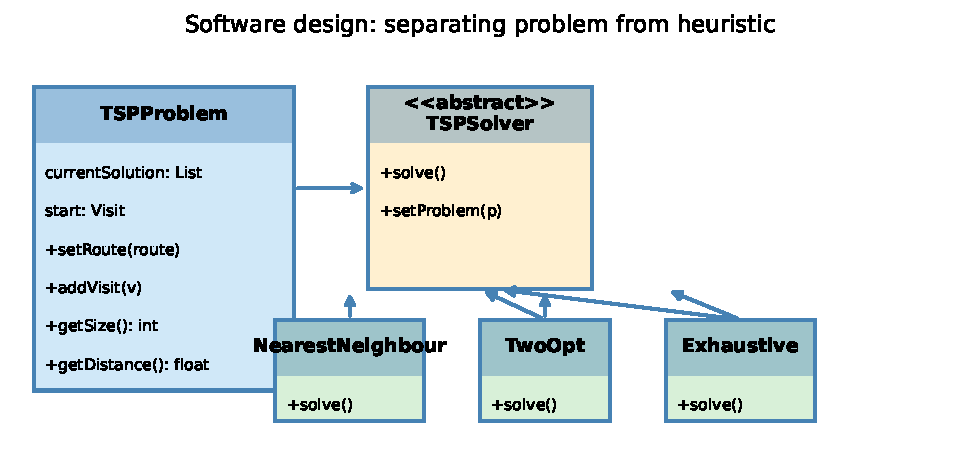
\includegraphics[width=0.80\textwidth]{fig_class_diagram.pdf}
    \caption{The TSP class hierarchy implementing the Strategy pattern.
    \texttt{TSPProblem} holds the data (cities, distance matrix, current
    solution).  \texttt{TSPSolver} is an abstract class with a
    \texttt{solve()} method.  Each concrete subclass
    (\texttt{NearestNeighbour}, \texttt{TwoOpt}, \texttt{Exhaustive})
    implements a different algorithm but is interchangeable through the
    common interface.}
  \end{figure}

\framebreak

  \textbf{Key design benefits.}

  \begin{itemize}
    \item \textbf{Extensibility:} Adding a new algorithm (e.g., 3-opt,
      a genetic algorithm) requires only adding a new subclass ---
      the rest of the system remains unchanged.
    \item \textbf{Testability:} Each algorithm can be unit-tested
      independently of the others.
    \item \textbf{Maintainability:} Domain experts writing heuristics do
      not need to understand the data-loading or distance-computation
      code, and vice versa.
    \item \textbf{Comparability:} By calling
      \texttt{solver.solve(problem)} with different solver objects, the
      case study can compare all algorithms on the same problem instance
      with minimal code change.
  \end{itemize}

  \medskip
  \textbf{Measuring distance: the Haversine formula.}
  The case study uses real-world geographic coordinates
  (latitude/longitude).  Straight-line Euclidean distance is
  inappropriate for a spherical Earth.  Instead, the
  \textbf{Haversine formula} computes the great-circle distance between
  two points:
  \[
    d = 2R \arcsin\!\left(
        \sqrt{
          \sin^2\!\left(\frac{\phi_2 - \phi_1}{2}\right)
          +
          \cos(\phi_1)\cos(\phi_2)\,
          \sin^2\!\left(\frac{\lambda_2 - \lambda_1}{2}\right)
        }
      \right)
  \]

  \begin{block}{Haversine notation}
    \begin{itemize}
      \item $\phi$ (phi): latitude in radians (the angle above the
        equator; ranges from $-\pi/2$ to $+\pi/2$).
      \item $\lambda$ (lambda): longitude in radians (the angle east of
        the prime meridian; ranges from $-\pi$ to $+\pi$).
      \item $R$: Earth's mean radius $\approx 6371$~km.
      \item $\arcsin$: the inverse sine function, returning an angle.
      \item The formula gives the shortest path over the surface of a
        sphere between two points.
    \end{itemize}
  \end{block}

  \begin{alertblock}{Key takeaway: software design}
    Separating the problem representation from the heuristic is not
    merely good style --- it makes the software genuinely easier to
    extend and compare.  This pattern will be reused in every chapter
    of the book.
  \end{alertblock}

\end{frame}

% ============================================================
\section{1.5~~A TSP Case Study: Santa Claus}
% ============================================================

\begin{frame}[allowframebreaks]{1.5~~A TSP Case Study: Santa's Delivery Problem}

  \textbf{Problem description.}
  The case study is a playful but technically rich problem: how should
  \textbf{Santa Claus} plan his sleigh route to deliver presents?

  Santa leaves his grotto in Lapland, visits the house of each child
  (one per country/region), delivers presents, and returns to the
  grotto.  The dataset contains 50~visits (children's locations)
  distributed across the world, with latitude/longitude coordinates.
  Santa uses the Haversine distance to measure how far apart any two
  locations are.

  \medskip
  \textbf{Goal.}
  Compare three algorithms --- \textbf{Exhaustive Search},
  \textbf{Nearest Neighbour}, and \textbf{2-opt} (and their hybrid
  combination) --- on instances of increasing size from 1 to 50~visits,
  measuring both \emph{solution quality} (total distance in~km) and
  \emph{execution time} (in~ms).

\framebreak

  \textbf{The Hybrid solver.}
  The best practical result is achieved by a \textbf{Hybrid} algorithm
  that first runs Nearest Neighbour to generate a reasonable initial
  tour, then applies 2-opt to improve it:

  \begin{figure}
    \centering
    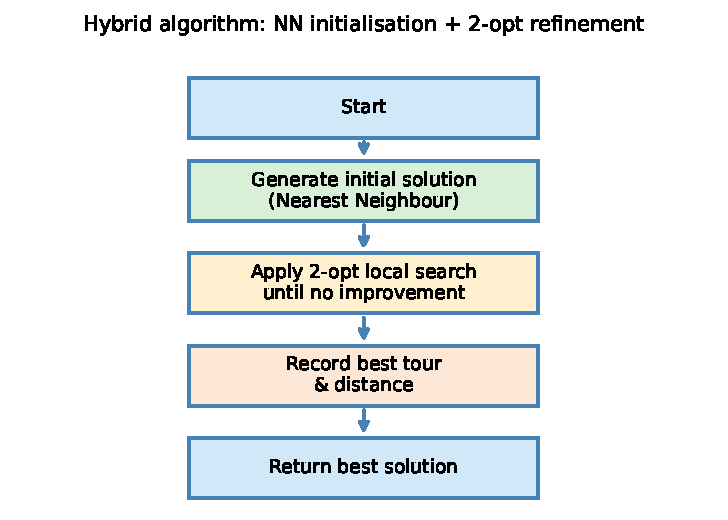
\includegraphics[width=0.45\textwidth]{fig_hybrid_flow.pdf}
    \caption{The Hybrid solver: NN builds an initial tour quickly;
    2-opt then iteratively refines it until no 2-edge swap gives further
    improvement.  This combination consistently outperforms either
    algorithm used alone.}
  \end{figure}

\framebreak

  \textbf{Experimental setup.}
  Each algorithm is run 10~times on each instance size, and the results
  are reported as \texttt{min(average)} over 10~runs.  For deterministic
  algorithms (Nearest Neighbour from a fixed start), only one run is
  needed.  The Exhaustive Search is excluded from instances with
  $n > 13$ cities because its running time becomes prohibitive.

\end{frame}

% ────────────────────────────────────────────────────────────
\begin{frame}[fragile]{Python: Exhaustive Search Algorithm}

\begin{lstlisting}[caption={Exhaustive search --- Python translation of the book's Java Listing 1.1}]
import itertools

def exhaustive_tsp(problem):
    """
    Enumerate every permutation of cities (fixing the start city)
    and return the shortest complete tour.
    problem.cities  : list of city objects
    problem.dist(a,b): distance between two cities
    """
    cities = problem.cities
    start  = cities[0]
    rest   = cities[1:]          # cities[1:] = all except the fixed start

    best_dist  = float('inf')    # infinity — will be beaten by any real tour
    best_route = None

    # itertools.permutations generates all (n-1)! orderings of rest
    for perm in itertools.permutations(rest):
        route = [start] + list(perm) + [start]  # complete circuit
        dist  = sum(problem.dist(route[i], route[i+1])
                    for i in range(len(route)-1))
        if dist < best_dist:     # found a shorter tour
            best_dist  = dist
            best_route = route

    return best_route, best_dist
\end{lstlisting}

\textbf{Code walkthrough.}
Line~10 uses \texttt{itertools.permutations} to generate every possible
ordering of the non-start cities without storing all permutations in
memory simultaneously.  Line~11 builds the complete circuit: start city,
then the permuted cities, then return to start.  Lines~12--13 compute
the tour length by summing the distances of all consecutive pairs.
Lines~14--16 update the best solution found so far.

\end{frame}

% ────────────────────────────────────────────────────────────
\begin{frame}[fragile]{Python: Nearest Neighbour Algorithm}

\begin{lstlisting}[caption={Nearest Neighbour heuristic --- Python translation of book Listing 1.2}]
def nearest_neighbour_tsp(problem):
    """
    Build a tour greedily: always go to the nearest unvisited city.
    Returns: (tour as list of cities, total distance)
    """
    cities    = problem.cities[:]   # copy so we can modify
    start     = problem.start       # fixed starting city
    current   = start
    route     = [current]
    not_visited = [c for c in cities if c != start]

    while not_visited:              # while there are unvisited cities
        best_d = float('inf')
        next_c = None
        for possible in not_visited:
            d = problem.dist(current, possible)
            if d < best_d:
                best_d = d
                next_c = possible   # closest unvisited city found so far
        not_visited.remove(next_c)  # mark as visited
        route.append(next_c)        # add to tour
        current = next_c            # move there

    route.append(start)             # return to start
    total = sum(problem.dist(route[i], route[i+1])
                for i in range(len(route)-1))
    return route, total
\end{lstlisting}

\textbf{Code walkthrough.}
Lines~10--11 initialise the list of unvisited cities (all except the
start).  The \texttt{while} loop (lines~13--21) continues until all
cities are visited.  Lines~14--18 scan every unvisited city for the
closest one.  Line~19 removes the chosen city from the unvisited list;
line~21 advances the current position.  Lines~23--25 close the circuit
and compute the total distance.

\end{frame}

% ────────────────────────────────────────────────────────────
\begin{frame}[fragile]{Python: 2-opt Algorithm}

\begin{lstlisting}[caption={2-opt heuristic --- Python translation of book Listing 1.3}]
def two_opt_swap(route, i, j):
    """
    Reverse the sub-sequence between positions i and j (inclusive).
    route: list of city objects (does NOT include return-to-start)
    """
    return route[:i] + route[i:j+1][::-1] + route[j+1:]

def two_opt_tsp(problem):
    """
    Improve an initial (e.g. NN) tour by repeatedly applying 2-opt swaps.
    """
    route = nearest_neighbour_tsp(problem)[0][:-1]  # remove trailing start
    improved = True

    while improved:                 # keep scanning until no swap helps
        improved = False
        best_dist = problem.get_distance(route)

        for i in range(len(route)):
            for j in range(i+1, len(route)):
                new_route = two_opt_swap(route, i, j)
                new_dist  = problem.get_distance(new_route)
                if new_dist < best_dist:   # improvement found
                    route     = new_route
                    best_dist = new_dist
                    improved  = True
                    break               # restart the scan
            if improved:
                break

    route.append(route[0])          # close the circuit
    return route, problem.get_distance(route[:-1])
\end{lstlisting}

\textbf{Code walkthrough.}
The helper \texttt{two\_opt\_swap} (lines~1--6) uses Python slice
notation: \texttt{route[i:j+1][::-1]} reverses the sub-list from
index~\texttt{i} to~\texttt{j}.
The main function starts from a NN tour (line~9).
The outer \texttt{while} loop (lines~13--28) runs until no improvement
is found.  The double \texttt{for} loop (lines~18--19) tries all
$\binom{n}{2}$ pairs.  Lines~22--25 accept the swap if it shortens the
tour and restart the scan.

\end{frame}

% ────────────────────────────────────────────────────────────
\begin{frame}[allowframebreaks]{1.5~~Results and Analysis}

  \textbf{Tour quality comparison.}
  The figure below shows the best tour distance found by each algorithm
  as the number of visits increases from 1 to 50.

  \begin{figure}
    \centering
    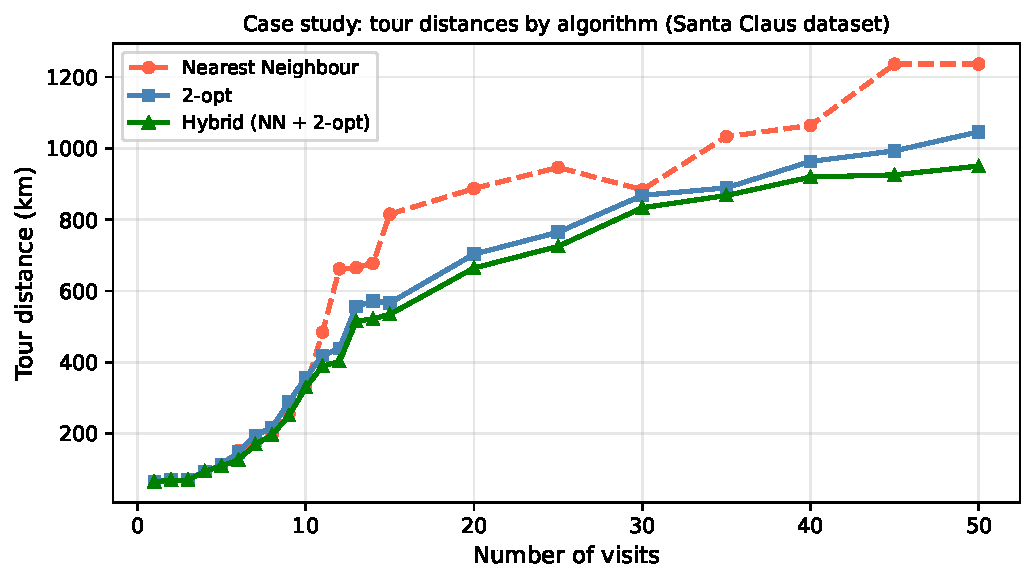
\includegraphics[width=0.80\textwidth]{fig_results_comparison.pdf}
    \caption{Tour distance vs.\ instance size for the three algorithms
    on the Santa Claus dataset.  The Hybrid solver (NN + 2-opt) gives
    the shortest tours for all instance sizes above 10~visits.
    For small instances ($n \leq 13$) the Exhaustive Search found the
    proven optimum.}
  \end{figure}

\framebreak

  \textbf{Numerical results (Table~1.3 from the book).}

  \begin{table}[htb]
  \centering
  \scriptsize
  \caption{Best tour distances (km) for the three algorithms.  Values in
  \textbf{bold} mark the best solution found for each instance size
  across all three methods.}
  \begin{tabular}{rrrr}
    \toprule
    Visits & Nearest Neighbour & 2-opt & Hybrid \\
    \midrule
    1  & \textbf{64.11}  & \textbf{64.11}  & \textbf{64.11}  \\
    5  & 112.35          & \textbf{111.04} & \textbf{108.77} \\
    10 & 328.77          & 356.88          & \textbf{328.77} \\
    15 & 677.64          & 566.39          & \textbf{534.40} \\
    20 & 815.50          & 676.26          & \textbf{664.34} \\
    25 & 887.28          & 725.15          & \textbf{725.15} \\
    30 & 946.70          & 868.17          & \textbf{833.44} \\
    35 & 883.80          & \textbf{834.98} & 867.89          \\
    40 & 1032.79         & 930.99          & \textbf{919.61} \\
    45 & 1064.67         & 934.25          & \textbf{925.88} \\
    50 & 1236.75         & 976.81          & \textbf{950.49} \\
    \bottomrule
  \end{tabular}
  \end{table}

  Notice that at $n = 35$ the pure 2-opt result ($834.98$) is
  \emph{slightly better} than the Hybrid ($867.89$).  This illustrates
  an important point: because the Hybrid starts from an NN solution
  that may differ between runs, it does not always dominate 2-opt
  started from a different random solution.  Averaging over multiple
  runs would smooth out such anomalies.

\framebreak

  \textbf{Execution time comparison.}

  From Table~1.2: Nearest Neighbour runs in under 1~ms for all instance
  sizes tested ($n \leq 50$).  2-opt takes 46~ms for $n = 50$.  The
  Hybrid requires 8.1~ms for $n = 50$ --- faster than pure 2-opt because
  the NN starting solution is already reasonably good, so 2-opt converges
  in fewer passes.

  \medskip
  \begin{exampleblock}{Interpretation of the Santa Claus results}
    The Hybrid solver achieves the best tour quality in 8.1~ms for
    50~visits --- a route of 950~km.  The na\"{\i}ve Nearest Neighbour
    produces a 1237~km route in under 1~ms.  The 30\% improvement in
    distance (from 1237~km to 950~km) delivered by the Hybrid at a cost
    of only 8~ms is a compelling illustration of why combining a fast
    construction heuristic with a local search improvement step is such
    a popular strategy in practice.
  \end{exampleblock}

  \begin{alertblock}{Three observations about the solvers}
    \begin{enumerate}
      \item Nearest Neighbour is fast but its tour quality degrades
        noticeably relative to 2-opt as $n$ grows.
      \item Pure 2-opt (started from a random solution) is slower than
        the Hybrid because a random starting tour is poor; the algorithm
        needs many more improvement passes.
      \item The Hybrid (NN + 2-opt) is the best choice: it leverages NN's
        speed to get a good starting point, then uses 2-opt to refine it.
    \end{enumerate}
  \end{alertblock}

\end{frame}

% ============================================================
\section{1.6~~Conclusions}
% ============================================================

\begin{frame}[allowframebreaks]{1.6~~Conclusions}

  \textbf{What we have learned in Chapter~1.}

  \medskip
  \textbf{The TSP is the canonical hard delivery problem.}
  Any problem that requires visiting a set of locations optimally is, at
  its core, a TSP or a variant of it.  Understanding the TSP --- its
  complexity, its solution methods, and its software design --- provides
  the foundation for every subsequent chapter.

  \medskip
  \textbf{The combinatorial explosion is the fundamental difficulty.}
  The number of possible routes grows as $(n-1)!/2$.  For $n = 20$
  cities this is already $6 \times 10^{16}$, making exhaustive search
  completely impractical.  This is why heuristics are not a compromise
  but a \emph{necessity}.

  \medskip
  \textbf{NP-hardness explains why no ``perfect'' polynomial-time
  algorithm exists.}
  Unless P = NP (which is widely believed to be false), the TSP cannot
  be solved exactly in polynomial time.  The best exact algorithms
  (Branch and Bound, Concorde) use clever bounding and cutting-plane
  techniques but still require exponential time in the worst case.

  \medskip
  \textbf{Heuristics provide practical solutions in reasonable time.}
  Nearest Neighbour runs in $O(n^2)$ and gives tours roughly 20--25\%
  above optimal.  2-opt (also $O(n^2)$ per pass) systematically removes
  crossing edges and reduces tour length by a further 10--20\%.
  Combining them (Hybrid: NN + 2-opt) consistently gives the best
  practical results and runs in milliseconds for 50~cities.

\framebreak

  \textbf{Software design matters as much as the algorithm.}
  Separating the \emph{problem} (the \texttt{TSPProblem} class with city
  data and distance computation) from the \emph{solver} (the abstract
  \texttt{TSPSolver} class and its concrete subclasses) follows the
  Strategy pattern.  This design makes it easy to add new algorithms,
  compare them fairly, and maintain the codebase as the project grows.

  \medskip
  \textbf{Looking ahead.}
  The methods studied in Chapter~1 are foundational, but they have
  limitations: 2-opt gets stuck in local optima, and the Hybrid has no
  mechanism to escape them.  The remaining chapters introduce
  \emph{nature-inspired metaheuristics} --- Evolutionary Algorithms,
  Ant Colony Optimisation, and others --- that use population-based or
  stochastic acceptance strategies to explore the solution space more
  broadly and find higher-quality solutions on large, real-world
  delivery instances.

  \begin{block}{Chapter summary in one sentence}
    The TSP captures the core difficulty of delivery optimisation ---
    NP-hard combinatorial search --- and the Nearest Neighbour plus 2-opt
    heuristics provide a fast, practical baseline that later
    nature-inspired methods aim to surpass.
  \end{block}

\end{frame}

% ── References ──────────────────────────────────────────────
\begin{frame}[allowframebreaks]{References}

  \begin{itemize}
    \item \textbf{Applegate, D., Bixby, R., Chv\'atal, V., Cook, W.}
      (2006).  \emph{The Traveling Salesman Problem: A Computational
      Study}.  Princeton University Press.

    \item \textbf{Bocks} (1958).  Solving the TSP on an IBM~650 computer.

    \item \textbf{Croes, G.A.} (1958).  A method for solving
      traveling-salesman problems.  \emph{Operations Research}, 6(6),
      791--812.

    \item \textbf{Flood, M.M.} (1956).  The traveling-salesman problem.
      \emph{Operations Research}, 4(1), 61--75.

    \item \textbf{Hamilton, W.R.} (1857).  The Icosian Game.  Exhibited
      at the British Association.

    \item \textbf{Lin, S., Kernighan, B.W.} (1973).  An effective
      heuristic algorithm for the traveling-salesman problem.
      \emph{Operations Research}, 21(2), 498--516.

    \item \textbf{OpenStreetMap contributors} (2021).  OpenStreetMap.
      \url{https://www.openstreetmap.org/copyright}

    \item \textbf{Springer} (2022).  \emph{Nature Inspired Optimisation
      for Delivery Problems}.  Studies in Computational Intelligence.
  \end{itemize}

\end{frame}

\end{document}
